\documentclass[a4paper,11pt,UTF8]{article}
\usepackage{ctex}
\usepackage{amsmath,amsthm,amssymb,amsfonts}
\usepackage{amsmath}
\usepackage[a4paper]{geometry}
\usepackage{graphicx}
\usepackage{microtype}
\usepackage{siunitx}
\usepackage{booktabs}
\usepackage[colorlinks=false, pdfborder={0 0 0}]{hyperref}
\usepackage{cleveref}
\usepackage{esint} 
\usepackage{graphicx}
\usepackage{ragged2e}
\usepackage{pifont}
\usepackage{extarrows}
\usepackage{mathptmx}
\usepackage{float}
\usepackage{caption}
\captionsetup[figure]{name={Figure}}
%opening
\title{模电知识点汇总}
\author{Yuejin Xie \quad U202210333}
\date{}
\begin{document}
\maketitle
At the beginning, the theories of all kinds of elements are unnecessary, you just need to know how to solve out the problems, that's the point.
\section{Op-Amp}
5 basic Op-Amp models:

\begin{figure}[H]
	\begin{minipage}{.69\textwidth}
		\begin{figure}[H] 
			\centering 
			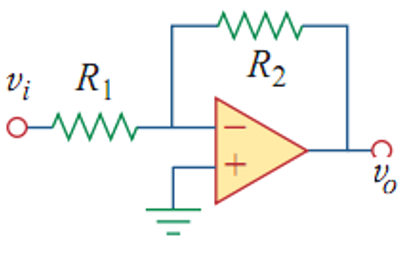
\includegraphics[scale=0.5]{./img/9.1.png}
			\caption{Inverting Amplifier}
		\end{figure}
	\end{minipage}
	\begin{minipage}{.29\textwidth}
		\LARGE{$$
			v_o=-\frac{R_2}{R_1}v_i
			$$}
	\end{minipage}
\end{figure}

\begin{figure}[H]
	\begin{minipage}{.5\textwidth}
		\begin{figure}[H] 
			\centering 
			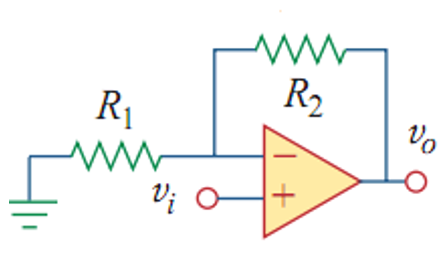
\includegraphics[scale=0.5]{./img/9.2.png}
			\caption{Inverting Amplifier}
		\end{figure}
	\end{minipage}
	\begin{minipage}{.5\textwidth}
		\LARGE{$$
			v_o=(1+\frac{R_2}{R_1})v_i
			$$}
	\end{minipage}
\end{figure}

\begin{figure}[H]
	\begin{minipage}{.5\textwidth}
		\begin{figure}[H] 
			\centering 
			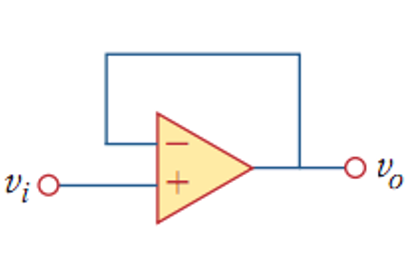
\includegraphics[scale=0.5]{./img/9.3.png}
			\caption{Inverting Amplifier}
		\end{figure}
	\end{minipage}
	\begin{minipage}{.5\textwidth}
		\LARGE{$$
			v_o=v_i
			$$}
	\end{minipage}
\end{figure}

\begin{figure}[H]
	\begin{minipage}{.5\textwidth}
		\begin{figure}[H] 
			\centering 
			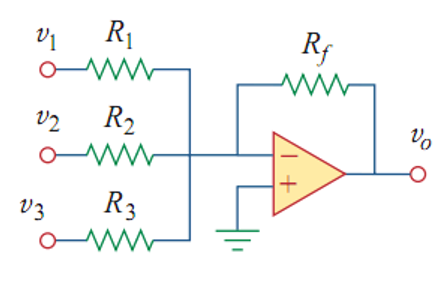
\includegraphics[scale=0.5]{./img/9.4.png}
			\caption{Inverting Amplifier}
		\end{figure}
	\end{minipage}
	\begin{minipage}{.5\textwidth}
		\LARGE{$$
			v_o=-(\frac{R_f}{R_1}v_1+\frac{R_f}{R_2}v_2+\frac{R_f}{R_3}v_3)
			$$}
	\end{minipage}
\end{figure}

\begin{figure}[H]
	\begin{minipage}{.5\textwidth}
		\begin{figure}[H] 
			\centering 
			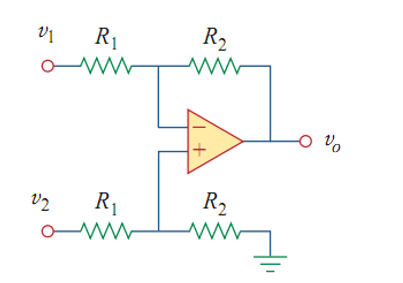
\includegraphics[scale=0.5]{./img/9.5.png}
			\caption{Inverting Amplifier}
		\end{figure}
	\end{minipage}
	\begin{minipage}{.5\textwidth}
		\LARGE{$$
			v_o=\frac{R_2}{R_1}(v_2-v_1)
			$$}
	\end{minipage}
\end{figure}
\section{Basic Diode}
The theory of diodes is PN junction, OK, that's not matter. The most import is the 4 models of Diode: ideal model, case 1 model, case 2 model, small signal model.

We first introduce the $i_D-v_D$ relationship:
$$
	i_D=I_S(e^{\frac{v_D}{nV_T}}-1)
$$
In this equation: $n$-ideality factor(for ideal diode, $n=1$), $I_S$-reverse-bias saturation current, $V_T$-thermal voltage at room temperature(In general, $V_T =0.026$V). And at the turning point, we define: $V_\gamma$-turn-on or cut-in voltage.

Now we introduce the 4 diode model:

\textbf{Ideal model:} the conduction voltage drop equals 0($V_\gamma=0$), and When reverse bias, the resistor is $\infty$
\begin{figure}[H]
	\begin{minipage}{.5\textwidth}
		\begin{figure}[H] 
			\centering 
			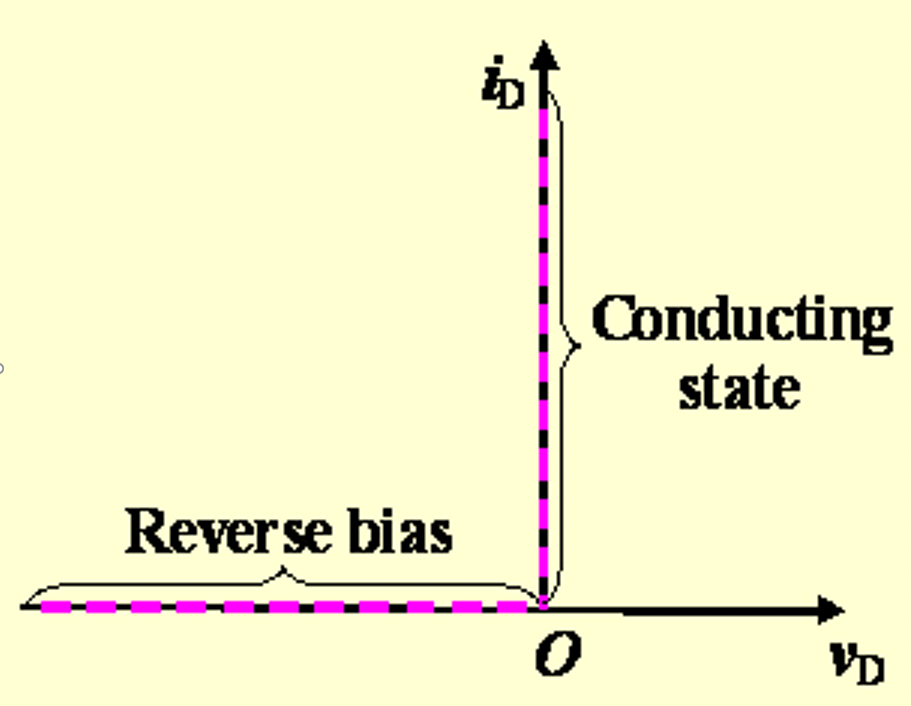
\includegraphics[scale=0.2]{./img/1.1}
			\caption{Inverting Amplifier}
		\end{figure}
	\end{minipage}
	\begin{minipage}{.5\textwidth}
		\LARGE{$$
			V_\gamma=0, r_d=\infty
			$$}
	\end{minipage}
\end{figure}
\textbf{Case 1 model:} consider conduction voltage drop($V_\gamma=0.6~0.7$V), when reverse bias, it's the same as the ideal model
\begin{figure}[H]
	\begin{minipage}{.5\textwidth}
		\begin{figure}[H] 
			\centering 
			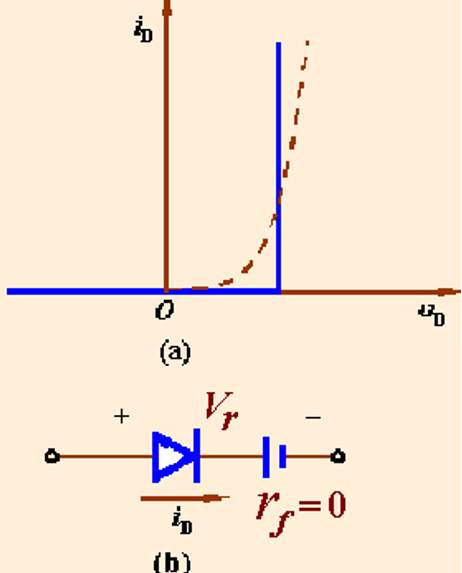
\includegraphics[scale=0.4]{./img/1.2}
			\caption{Inverting Amplifier}
		\end{figure}
	\end{minipage}
	\begin{minipage}{.29\textwidth}
		\LARGE{$$
			V_\gamma=0.6~0.7\mathrm{V}, r_d=\infty
			$$}
	\end{minipage}
\end{figure}
\textbf{Case 2 model:} consider conduction voltage drop Forward diode resistance, when reverse bias, it's the same as the ideal model.
\begin{figure}[H]
	\begin{minipage}{.5\textwidth}
		\begin{figure}[H] 
			\centering 
			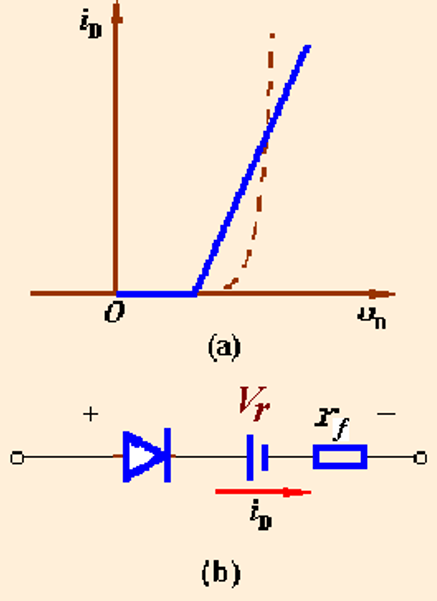
\includegraphics[scale=0.4]{./img/1.3}
			\caption{Inverting Amplifier}
		\end{figure}
	\end{minipage}
	\begin{minipage}{.5\textwidth}
		\LARGE{$$
			V_\gamma=0.6~0.7\mathrm{V}, r_d\neq\infty
			$$}
	\end{minipage}
\end{figure}
\textbf{Small signal model:} it's a model use for AC analysis. When a diode is operating in the small range,it can be a small-signal incremental resistance:
$$
	r_d=\frac{\Delta v_D}{\Delta i_D}
$$

We have equation:$\displaystyle i_D=I_S(e^{\frac{v_D}{V_T}}-1)$, therefore:
$$\begin{aligned}
	g_d&=\left.\frac{\mathrm{d}i_D}{\mathrm{d}v_D}\right|_Q=\left.\frac{I_Se^{\frac{v_D}{V_T}}}{V_T}\right|_Q=\left.\frac{I_{DQ}}{V_T}\right|_Q(e^{\frac{v_D}{V_T}}\approx e^{\frac{v_D}{V_T}}-1)\\
	\Rightarrow r_d&=\left.\frac{V_T}{I_{DQ}}\right|_Q
\end{aligned}	
$$
\begin{figure}[H]
	\begin{minipage}{.5\textwidth}
		\begin{figure}[H] 
			\centering 
			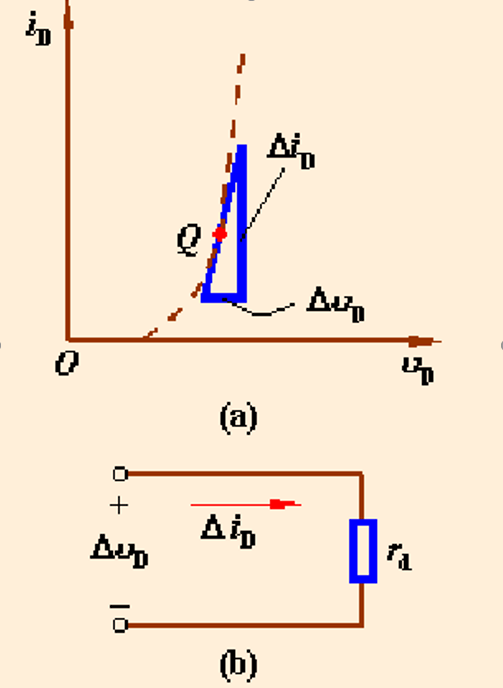
\includegraphics[scale=0.4]{./img/1.4}
			\caption{Inverting Amplifier}
		\end{figure}
	\end{minipage}
	\begin{minipage}{.5\textwidth}
		\LARGE{$$
			V_\gamma=0.6-0.7\mathrm{V}, r_d=\left.\frac{V_T}{I_{DQ}}\right|_Q
			$$}
	\end{minipage}
\end{figure}
\section{Other Diodes}
To analyze diode, The most important thing is to discuss all cases of diode, and you may need to consider conductivity of different diodes.

\textbf{Half-Wave Rectifier} Just Diode

\textbf{Full-Wave Rectifier}:

\textbf{\quad1.Rectifier with center-tapped transformer}
\begin{figure}[H]
	\begin{minipage}{.5\textwidth}
		\begin{figure}[H] 
			\centering 
			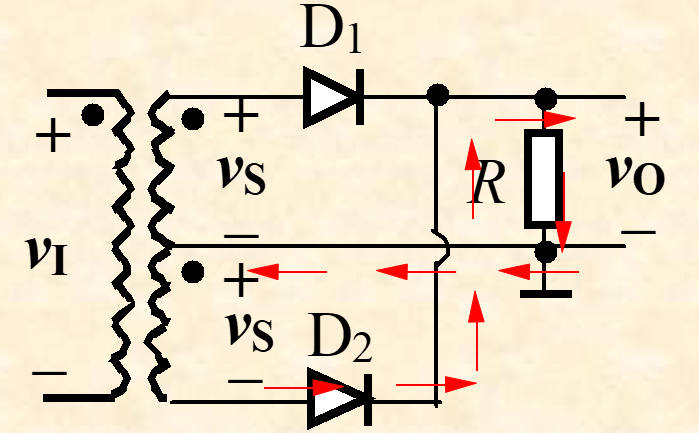
\includegraphics[scale=0.3]{./img/2.1}
			\caption{Inverting Amplifier}
		\end{figure}
	\end{minipage}
	\begin{minipage}{.5\textwidth}
		\begin{figure}[H] 
			\centering 
			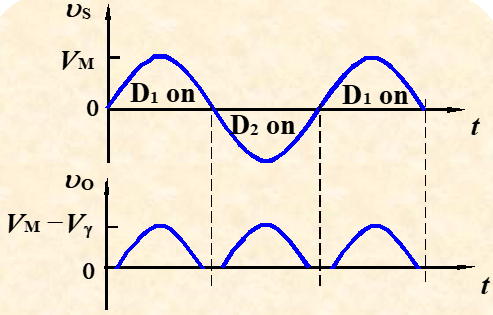
\includegraphics[scale=0.4]{./img/2.2}
			\caption{Inverting Amplifier}
		\end{figure}
	\end{minipage}
\end{figure}
\textbf{\quad2.Bridge eectifier}
\begin{figure}[H] 
	\centering 
	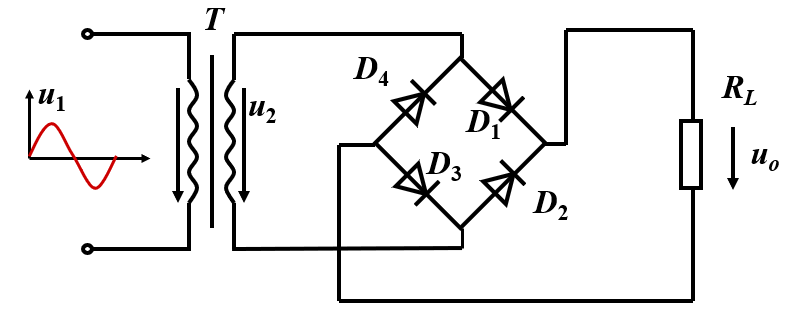
\includegraphics[scale=0.4]{./img/2.3}
	\caption{Inverting Amplifier}
\end{figure}
\textbf{Zener Diode:}
\section{MOSFET}

\section{BJT}

\section{Frequency Response}

\section{Power-Amplifier}



\end{document}